\documentclass[a4paper, 12pt]{article}
\usepackage[english]{babel}
\usepackage[utf8]{inputenc}
\usepackage[T1]{fontenc}
\usepackage{csquotes}
\usepackage{graphicx}
\usepackage{fancyhdr}
\usepackage{listings}
\usepackage{xcolor}
\usepackage[textsize=tiny]{todonotes}
\usepackage[style=ieee, backend=biber]{biblatex}
\usepackage{hyperref}

\setlength {\marginparwidth }{2cm}

% Code listing style
\definecolor{codegreen}{rgb}{0,0.6,0}
\definecolor{codegray}{rgb}{0.5,0.5,0.5}
\definecolor{codepurple}{rgb}{0.68,0,0.92}
\definecolor{backcolour}{rgb}{0.95, 0.95, 0.95}
\definecolor{codeblue}{rgb}{0.2,0.4,1}
\lstdefinestyle{mystyle}{
    language=C,
    morekeywords={diff_op_t},
    backgroundcolor=\color{backcolour}, 
    commentstyle=\color{codegray},
    keywordstyle=\color{codepurple},
    stringstyle=\color{codegreen},
    % identifierstyle=\color{codeblue},
    basicstyle=\ttfamily\footnotesize,
    breakatwhitespace=false,
    breaklines=true,
    captionpos=b,
    keepspaces=true,
    numbersep=5pt,
    showspaces=false,
    showstringspaces=false,
    showtabs=false,
    tabsize=2
}
\lstset{style=mystyle}


% Bibliography
\addbibresource{sources.bib}

% Title page
\pagestyle{fancy}
\fancyhf{}
\lhead{Uppsala University}
\cfoot{\thepage}
\renewcommand{\headrulewidth}{0.5pt}
\renewcommand{\footrulewidth}{0.5pt}
\setlength{\headheight}{15pt}

\begin{document}


\begin{titlepage}

\begin{figure}
    \begin{center}
        
\includegraphics[scale=0.5]{img/UU_LOGO.png}
    \end{center}
\end{figure}

\thispagestyle{fancy}

\vspace{1in}

\center

\textsc{\large BACHELOR THESIS REPORT} %Change to Bachelor if applicable

\vspace{0.5in}

\noindent\makebox[\linewidth]{\rule{\linewidth}{1.2pt}}
\textsc{ \textbf{\large 
Dynamic Software Updates in Embedded Devices
}}
\noindent\makebox[\linewidth]{\rule{\linewidth}{1.2pt}}

\vspace{0.5in}

\begin{minipage}{0.48\textwidth}
    \begin{flushleft}
        \textit{Student:} \\
        Arvid Morelid    \\
        arvid.morelid.5203@student.uu.se \\
    \end{flushleft}
\end{minipage}
\begin{minipage}{0.48\textwidth}
    \begin{flushright}
    \textit{Supervisor:} \\
    Ahmed El Yaacoub \\
    ahmed.el.yaacoub@angstrom.uu.se   \\
    \end{flushright}
\end{minipage}

\vspace{.5in}
\begin{minipage}{.97\textwidth}
    \begin{flushleft}
        \textit{Subject Reviewer:} \\
        Thiemo Voigt \\
        thiemo.voigt@angstrom.uu.se \\
    \end{flushleft}
\end{minipage}

\vspace{.5in}

\textbf{\large Department of Information Technology} \\

\today

\end{titlepage}

\newpage


\setcounter{page}{2}
\tableofcontents
\newpage

% Todo-list
\listoftodos
% Start of the report
\section*{Abstract}
Dynamic Software Updates (DSU) enable a system to be updated while it is running, ensuring that the system remains available and operational all the while providing increased security and correctness. However, the current literature on DSU in embedded systems with real-time requirements is limited, and it is a space where DSU may provide significant benefits. 

This paper presents an implementation of Dynamic Software Updates targeting real-time systems, utilising Ferroelectric Random Access Memory (FRAM) as the main memory technology. FRAM promises to outperform traditional storage mediums such as Flash, and this research provides insight into the potential benefits and drawbacks of using FRAM for DSU in embedded systems. 

The experimental results along with proof-of-concept updates on a real application show that the proposed method can perform updates with minimal overhead, ensuring that real-time deadlines are met. The research also provides a comparison between the performance of FRAM and Flash, showing that FRAM can provide significant benefits in terms of update time and energy efficiency.

\textbf{\textit{Keywords:}} Dynamic Software Updates, Real-time Systems, FRAM


\section{Introduction}
Traditionally, software updates in embedded systems have been approached with a model that involves taking the system offline for a brief period. While this approach is feasible for many applications, there exists a subset of embedded systems where downtime is not an option due to the critical nature of their operations. These systems operate in environments where interruptions can result in severe consequences, including compromised safety, financial losses, or disruptions to essential services. Examples of these systems include aerial drones and other mobile robots, automotive systems, power generation facilities and smart grids. An alternative to the traditional approach is DSU (Dynamic Software Updates), where the system is updated while it is running. This approach allows for the system to continue operating during the update process, ensuring that the system remains available and operational by eliminating overhead time in terms of boot and initialization of the software. The DSU approach does not however come without its challenges, as the update process must be performed in a manner that does not compromise the system's integrity, safety, or real-time deadlines.

While the concept of dynamic software updates is not new, there have been little research on utilising DSU in embedded systems with real-time requirements. With the wide variety of microcontroller architectures and operating systems present, the challenges of implementing DSU in embedded systems are many. But this diversity also presents opportunities for developing new methods and techniques for performing DSU. One such opportunity which this project aims to investigate is the use of Ferroelectric Random-access Memory (FRAM). FRAM is a non-volatile memory technology that has the potential to outperform traditional storage such as EEPROM and Flash in such scenarios, and is further described in section \ref{sec:platform}.

Previous work in the field have targeted different methods of performing the updates, such as Holmbacka et al. \cite{dynUpdateFramework} who provide a framework to perform updates by dynamically relinking FreeRTOS tasks. This approach was shown to add overhead in the magnitude of 10s of milliseconds. On the other hand, Yaacoub et al. \cite{NeRTA} present a method to schedule the dynamic updates in a manner such that real-time deadlines can be met by analysing and predicting idle processor time. They recorded a maximum idle time of just under 3ms when measuring on a low level flight controller, Hackflight \cite{hackflight}. This shows that some use cases may present overhead restrictions far lower than those measured by Holmbacka et al. and the necessity to investigate other methods for performing the update. This thesis project aims to investigate methods for dynamic software updates, targeting these tighter real-time deadlines. 



\section{Related Work}
As previously mentioned, DSU in embedded and real time systems is relatively under-represented in the literature. However, there are some studies which have investigated the topic, and some of these are discussed in this section.

One study by Wahler et al. \cite{dynUpdateFramework} introduce a framework for developing DSU-friendly systems in embedded devices. Their framework is based on dividing the system into components which can be swapped out independently of one another, providing a high degree of flexibility when it comes to DSU. They also show that their framework can meet real-time deadlines as small as 3.3ms including a state transfer of a  4000 byte state.  Their approach is promising, but the processor used in the experiments is a 32-bit MPC5200 running at 396MHz, which is significantly more powerful than the MSP430FR5994 used in this research. Thus, it is not clear how the results would translate to a less powerful system with more stringent real-time requirements.

Another study by Kilpeläinen \cite{Kilpelainen2023} present a thorough theoretical analysis of DSU in embedded systems. They propose a method for performing DSU in systems with Flash memory, which is a common storage medium in embedded systems. Their method involves copying the page to be updated into a buffer in RAM, where the changes are applied, and then erasing and rewriting the page. The proposed solution has some similarities to the solution presented in this research, in that it utilises binary differencing (\textit{diffing}). Diffing may prove a more suitable solution for embedded systems as it is less memory intensive than component based solutions, which require multiple copies of the application to be stored in memory, at least temporarily. However, the approach presented by Kilpelainen2023 is not ideal for systems with real-time requirements, as it introduces significant time costs for the update process. The method is also not tested in a practical setting, so it is not clear how the solution would perform. 

The solution presented in this research is based on the idea of generating a patch file which describes the changes to be made to the binary image. Multiple studies which focus on the generation of a patch file for DSU have been conducted. One such example is \cite{dsuEnhancer}, where the authors Kim et al. present a system which generates a patch file for resource constrained systems. They propose a solution similar to this research, where the patch file generator is run off the target device, and is then applied after transfer. Their approach is to insert branch instructions into the old versions of functions, which jump to the new implementation. This approach is beneficial when it comes to reducing the runtime overhead of the update, but it is not clear how this affects memory utilisation. Since the old version of the binary is left on the device, it is possible that the memory overhead of the update is higher than in a system where the old version is removed. In addition, the system utilises dynamic memory allocation to store and apply the patch file, which is not ideal for a real-time embedded system, as it is inherently less predictable than static memory allocation. The system is also not tested on a real-time system, so it is not clear how the system would perform in a real-time environment.

A similar approach for patch file generation is presented by Felser et al. in \cite{resourceConstrained}. They analyse ELF files to find the differences between versions of the application and generate a patch file which describes the changes between the two versions. The patch file is generated off the target device, and they use a manager to schedule and distribute it across a network of embedded nodes. This approach is more granular than Kim et al. in \cite{dsuEnhancer}, and could prove more suitable as a complement to this research. The research again focuses on the patch file generation and application, but does not discuss the real-time requirements of the system. It is nevertheless an approach that could be used for automatic patch file generation in a system similar to this research.


\section{Background}
This section describes in further detail some key concepts that are relevant to the research, and provides a more detailed problem statement and requirements for the project.

\subsubsection*{The platform}\label{sec:platform}
The platform used for the experiments in this project is the Texas Instruments MSP430FR5994 16MHz microcontroller. The MSP430FR5994 features a 16-bit RISC architecture and is equipped with 256KB of FRAM (Ferroelectric Random Access Memory), 8KB of SRAM, and 2KB of flash memory. The relatively large FRAM is particularly useful for this project since it is a non-volatile memory which at the same time provides high speed writes and low power consumption. This comes as a result of FRAM being addressable in a bit-wise manner, although on the byte level in the code, as opposed to Flash memory or EEPROM which requires entire pages to be erased before new data can be written, slowing down the operations \cite{framReport}. A side-effect of FRAM being non-volatile is that the binary image of the program is stored in the same place that it is executed from, and can thus be updated in-place with little overhead.

FRAM is also a low power memory technology since it doesn't require a charge pump to write data, as opposed to Flash memory or EEPROM. This is particularly useful in battery-powered devices, where power consumption is a critical factor. In addition to the speed, power efficiency and non-volatility, FRAM also has a much higher endurance than Flash memory, with a specified $10^{15}$ write cycles \cite{framReport}. This makes it a suitable candidate for devices that are expected to run continuously for long periods of time, devices which would benefit greatly from the ability to update the software in the field.

One drawback of FRAM is that accesses to it are limited to 8MHz. Thus, if the microcontroller is running at 16MHz, the CPU will be stalled for every access to FRAM \cite{framReport}. This is a limitation that must be considered when measuring the performance of the update process. The wait states require no user interaction apart from the initial setup of the microcontroller, and are handled automatically by the CPU.

\textbf{\textit{Memory layout}}. The MSP430FR5994 uses a unified memory model where FRAM, SRAM and registers can be accessed in the same memory space. The memory layout of the MSP430FR5994 can be seen in table \ref{tab:memory_layout}.
\begin{table}
\centering
\begin{tabular}{|p{0.55\linewidth}|c|c|}
    \hline
    \textbf{Memory} & \textbf{Address range} & \textbf{Size} \\
    \hline
    Reserved, Tiny RAM, Peripherals & 0x0000-0x0FFF & 4KB \\
    \hline
    Bootloader memory (ROM) & 0x1000-0x17FF & 2KB \\
    \hline
    Information memory, Device Descriptor (FRAM) & 0x1800-0x1AFF & 768B \\
    \hline
    VACANT & 0x1B00-0x1BFF & 256B \\
    \hline
    \textbf{RAM} & \textbf{0x1C00-0x3BFF} & \textbf{8KB} \\
    \hline
    \textbf{Code and Data memory, Interrupt vectors (FRAM)} & \textbf{0x4000-0x43FFF} & \textbf{256KB} \\
    \hline
\end{tabular}
\caption{Memory layout of the MSP430FR5994 microcontroller \cite{fr5994DataSheet}.}
\label{tab:memory_layout}
\end{table}

The table has been simplified to highlight the important parts of discussion for this research. Essentially, the final section of the memory space is the main memory used in any application running on the device. This is where the binary image of the program is stored, and where the update process will take place. The memory space is automatically divided into two sections by the compiler and linker, FRAM (0x4000-0xFFFF) and HIFRAM (0x10000 - 0x43FFF). This is due to the fact that the 16-bit architecture of the microprocessor doesn't allow addressing beyond 16-bit memory addresses. Accessing the HIFRAM section is only possible with an extension of the instruction set, using less efficient, emulated instructions. How these sections are used is up to the developer and can be configured in the linker script. 

To facilitate an efficient update process, the program should be structured in such a way that the added or removed code affects the rest of the program as little as possible. For example, moving a function in memory requires that all calls to said function are updated, which can be a time-consuming process. Thus, in this research, the memory layout opted for is to have the DSU functionality in the FRAM section, with all other application code in the HIFRAM section. This way, the DSU code is never affected by the update process, which would be the case if it was stored in the same section as the application code. 

The drawback of this approach is that the program code is not as fast to access as it would be if it was stored in the FRAM section. This is a trade-off that was deemed necessary due to the decrease in complexity of any update performed.  

\subsubsection*{Problem statement}
As described in previous sections, DSU in embedded and real-time systems is not a new concept, but there are some key aspects that are yet to be considered in the field. 

Firstly; the currently existing work in the field of DSU have been focused on systems with more relaxed real-time requirements, where the overhead of the update process is not as critical. This project aims to investigate the use of DSU in systems with tighter real-time deadlines, where the overhead of the update process must be kept to a minimum.

Secondly; to meet these deadlines, the utilisation of FRAM is proposed as a potential solution, and this research aims to investigate the performance impact that the technology has on the update process.  

\subsubsection*{Requirements}
As a way of containing the scope of the project, and to provide a clear goal for the research, the requirements of the work need to be clearly defined. There are a multitude of requirements to consider in the context of DSU, both functional and non-functional. Mlinarić describes in \cite{dsuChallenges} five key requirements for any DSU implementation, namely: \textit{Availability}, \textit{Correctness}, \textit{Flexibility}, \textit{Performance}, and \textit{Simplicity}. In addition to these general requirements for DSU, there are also requirements that are specific to the context of embedded systems, which may be considered subcategories of the above; \textit{Energy efficiency}, \textit{Memory usage}, and \textit{Security}.
\todo{Maybe expand on these}

The main focus of this research is the performance of the update process, however other aspects such as security and correctness are considered when evaluating the results, as they are factors which may impact the performance, and thus, the feasibility of the solution.

\section{Method}
\subsection{The Platform}
The platform used for the experiments in this project is the Texas Instruments MSP430FR5994 microcontroller. The MSP430FR5994 features a 16-bit RISC architecture and is equipped with 256KB of FRAM (Ferroelectric Random Access Memory), 8KB of SRAM, and 2KB of flash memory. The relatively large FRAM is particularly useful for this project since it is a non-volatile memory which at the same time provides high speed writes and low power consumption. This comes as a result of FRAM being writeable in a bit-wise manner, as opposed to Flash memory or EEPROM which requires entire pages to be erased before new data can be written, slowing down the operations \cite{framReport}. A side-effect of FRAM being non-volatile is that the binary image of the program is stored in the same place that it is executed from, and can be done in-place with little overhead. 

\subsection{The update process}
The update process is initiated by sending a command to the microcontroller over a serial connection. The command is received by the microcontroller and triggers the update process. The update process is divided into three main steps: patch file generation [\ref{sec:patchfile}], updating, and the finalization. The following sections will describe each step in detail.

\subsubsection{Patch file generation}\label{sec:patchfile}
Another important part of the update process is the generation of the patch file. The patch file must be minimal in size to keep the transfer- and parse times within the expected idle time. This naturally excludes simply transferring the entire binary image as an option. Instead, a \textit{diff}-file is generated by a server system by comparing the current binary to the patched one. For sufficiently small updates, the diff file could be as simple as stating addresses to changed instructions and/or data, and the new values for said addresses. This is however not ideal in the case of bigger updates since changes could cause portions of the binary to be shifted, which can be expressed with a \textbf{Shift} operation instead of individual byte- or word-level changes. Thus, a better approach is to use a binary diffing tool such as \textit{BinDiff} to generate a patch file.

\todo{Describe problem of finding instruction addresses}




\section{Results}
This section presents the results of the experiments conducted in this project. The experiments were designed to evaluate the performance of the DSU process in the context of embedded systems, and to investigate the impact of using FRAM as the storage medium for the update process. The main focus of the experiments was to measure the time it takes to perform the update process, and evaluate if the procedure is feasible in a real-time system.

All of the below experiments were conducted on the MSP430FR5994 microcontroller, running at both 8MHz and 16MHz. The data was gathered using the built-in debugging tools of the Code Composer Studio IDE. The time estimates were not measured directly but instead calculated based on the number of clock cycles spent in each part of the update process, along with the clock frequency. 

\section{Simulated Updates}
As an in depth performance evaluation of the DSU process, a series of simulated updates were conducted. The simulated updates were designed to test the performance of the DSU process under various conditions, such as different update sizes, and using different clock frequencies. The simulated updates were conducted by manually creating \textit{diff} files and applying them to a preallocated array in the upper FRAM of the device. The simulated updates uses only one operation type each, to measure the impact of each operation. In the first series of experiments, the focus is to determine the bottlenecks of the process, as well as how to structure the \textit{diff} files to optimise performance. The second series of experiments focus on the clock frequency of the device, an important factor in deciding the usefulness of FRAM as the storage medium for the device.
\subsection{Decode and apply performance}
\subsubsection*{\textbf{\textit{Decode phase}}}
Figure \ref{fig:wDecode8} shows the processor cycles required to decode \textbf{Write} operations at different update sizes running at 8MHz. The cycles required to decode the operation is linear with the size of the update, and grows at an increasingly higher rate the more operations are used, as shown by the "1 op / Word" data points. This 'context switching' overhead is sizeable, adding triple the amount of cycles compared to extending a single operation with another word of data. This underlines the importance of minimizing the number of operations in an update.
\begin{figure}[!ht]
    \begin{shaded}
        \centering
        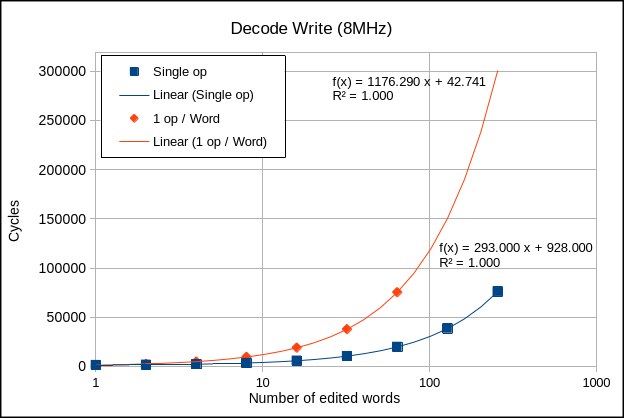
\includegraphics[width=\figurewidth]{img/WDecode8.png}
        \caption{Cycles required to decode \textbf{Write} operations running at 8MHz.}
        \label{fig:wDecode8}
    \end{shaded}
\end{figure}
The maximum update size tested was 256 words for a single operation, and a maximum of 64 operations at one word each. This is a limitation owing to the small amount of available SRAM on the device, limiting the size of the \textit{diff} file. Potential solutions to this limitation are discussed in Section \ref{sec:future_work}. 

Similarly to the \textbf{Write} operation, effort should be made to minimize the number of \textbf{Shift} operations for any given update. This is shown in figure \ref{fig:sDecode8}, where the number of cycles required to decode the operations grows even more rapidly with the number of operations. This, however, is not as critical as the \textbf{Write} operation, as the number of \textbf{Shift} operations is expected to be lower than the number of \textbf{Write} operations for a given update. 
\begin{figure}[!ht]
    \begin{shaded}
        \centering
        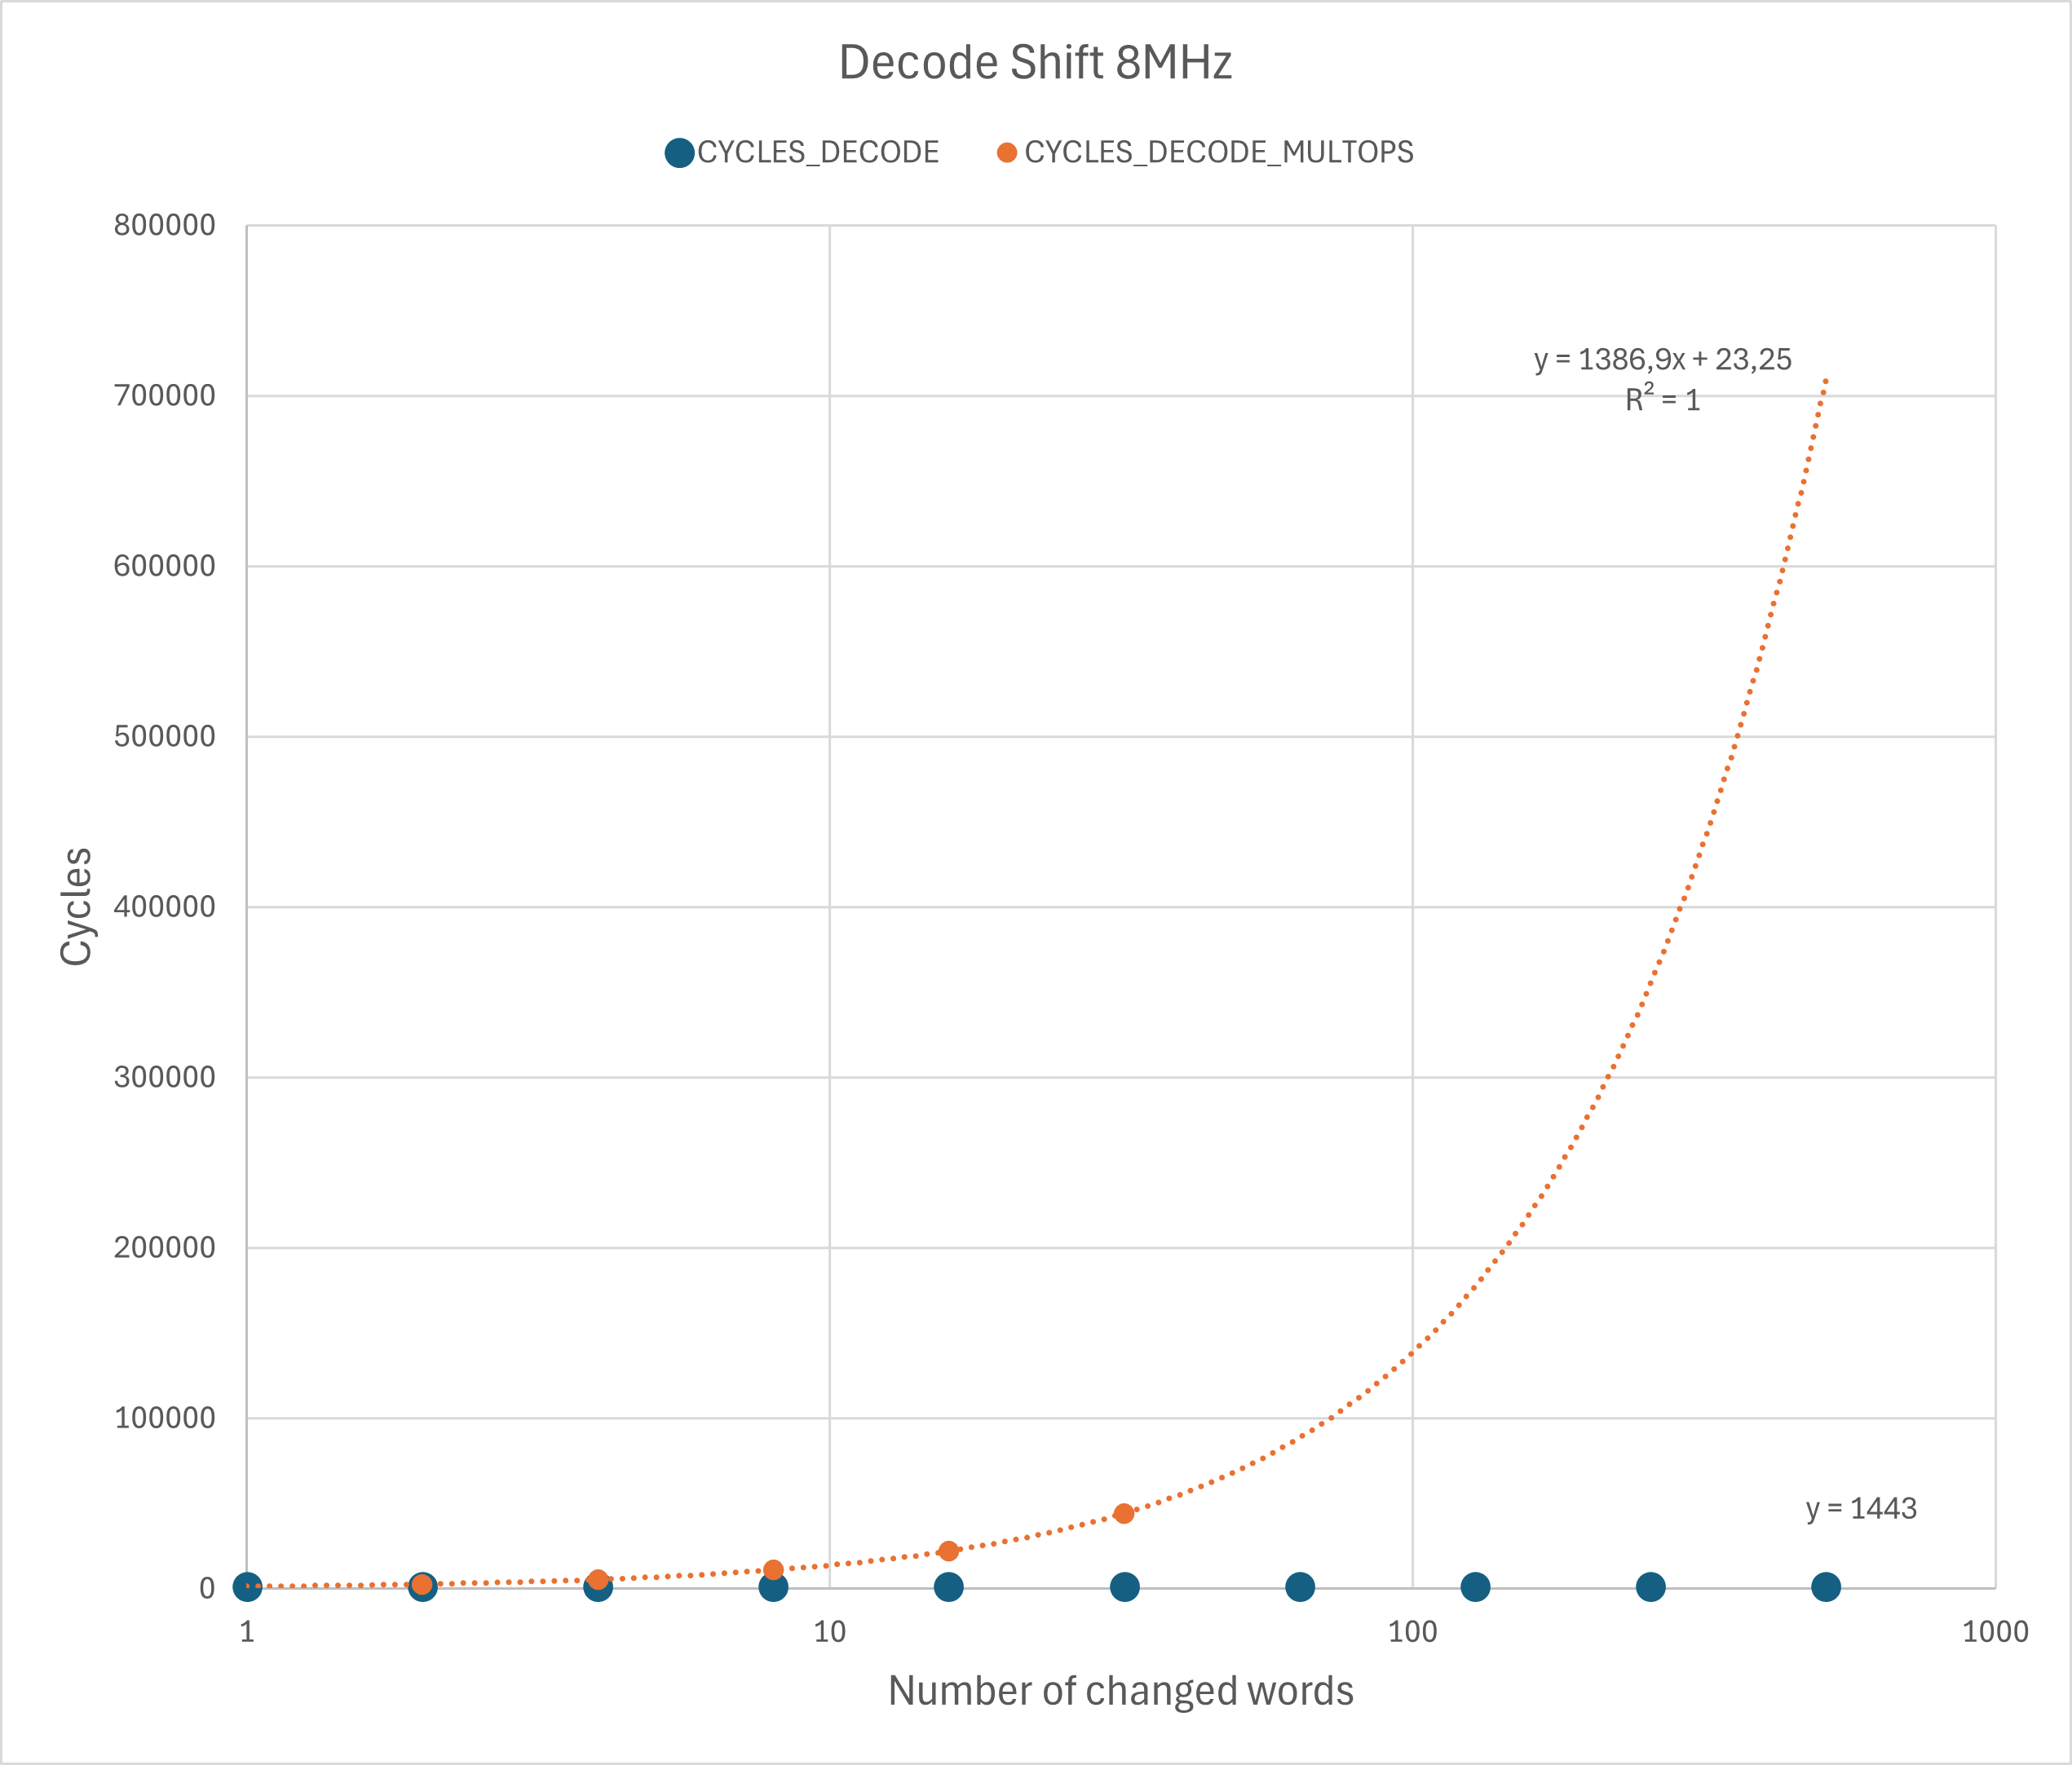
\includegraphics[width=\figurewidth]{img/SDecode8.png}
        \caption{Cycles required to decode \textbf{Shift} operations running at 8MHz.}
        \label{fig:sDecode8}
    \end{shaded}
\end{figure}
Again, the available RAM of the device limited the maximum update size tested to just 32 operations. 

The results of the simulated updates show that the decode phase is very taxing on the processor, and that the number of operations in an update has a significant impact on the time it takes to decode the update. The main focus of this research however, is the impact that the FRAM has on the performance of the update process. this is more clearly shown in the apply phase, where the use of, for example, Flash would bring a severe performance penalty.

\subsubsection*{\textbf{\textit{Apply phase}}}
Figure \ref{fig:wApply8} shows the \textit{application} of the previously discussed updates. The cycles required to apply the updates is also linear with the size of the update, but the rate of growth is significantly lower than that of the decode phase.
\begin{figure}[!ht]
    \begin{shaded}
        \centering
        \includegraphics[width=\figurewidth]{img/wApply8.png}
        \caption{Cycles required to apply \textbf{Write} operations running at 8MHz.}
        \label{fig:wApply8}
    \end{shaded}
\end{figure}
Here, a view of the improvement over traditional storage mediums can be seen. Using numbers from the data sheet for similar platforms from Texas Instruments, which use Flash \cite{msp430Flash}, the maximum speed for pre-erasing 512 bytes of data on Flash is 23ms, or an estimated 11.5ms for 256 bytes. This is well beyond the real-time deadlines which researchers such as Yaacoub et al. have shown to be realistic \cite{NeRTA}, and does not include the time it takes to write the data. In comparison, the DSU process using FRAM can write this data in just 0.44ms, as estimated from the data in figure \ref{fig:wApply8}, nearly two order of magnitude faster.

The \textbf{Shift} operation behaves identically when it comes to the apply phase, as seen in figure \ref{fig:sDecodeVsApply}. The growth of 12 cycles for each additional edited word, with a fixed decode cost, means the \textbf{Shift} operation allows updates which shift large portions of the code without significant performance costs. Using the linear equation from the figure, $f(x)=12x+134$, an approximate 1988 words, or 3976 bytes could be written or shifted within 3ms. 
\begin{figure}[!ht]
    \begin{shaded}
        \centering
        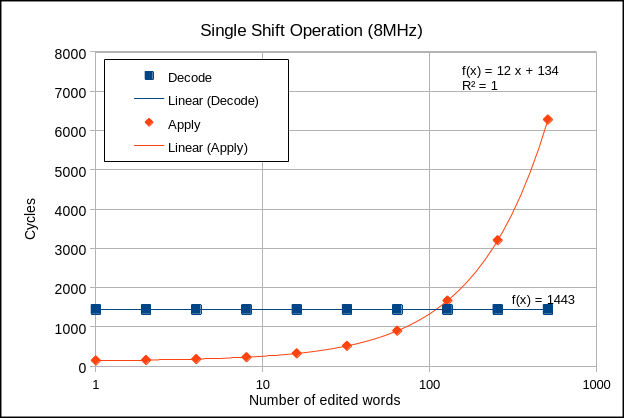
\includegraphics[width=\figurewidth]{img/SDecodeVsApply.png}
        \caption{Comparison of Decode and Apply phases for a single \textbf{Shift} operation running at 8MHz.}
        \label{fig:sDecodeVsApply}
    \end{shaded}
\end{figure}
Additional tests were made to verify that the \textit{offset} of the \textbf{Shift} operation does not impact the performance, and the results showed that this is indeed the case. 

\subsection{Clock frequency impact}
As previously mentioned, the MSP430FR5994 is limited to 8MHz when accessing FRAM. This means running the device at 16MHz will require wait states for every access to FRAM. Although this introduces some overhead in the form of additional cycles required for each access, the overall real-time performance of the update process should still be improved owing to the faster processing of data.  
In Figure \ref{fig:w8vs16}, the difference in required cycles can be seen when running the same update at different clock frequencies. Even with the added overhead of wait state cycles, the update process is faster at 16MHz than at 8MHz, running at twice the speed but with, on average, $22.9\%$ more cycles required. 
\begin{figure}[!ht]
    \begin{shaded}
        \centering
        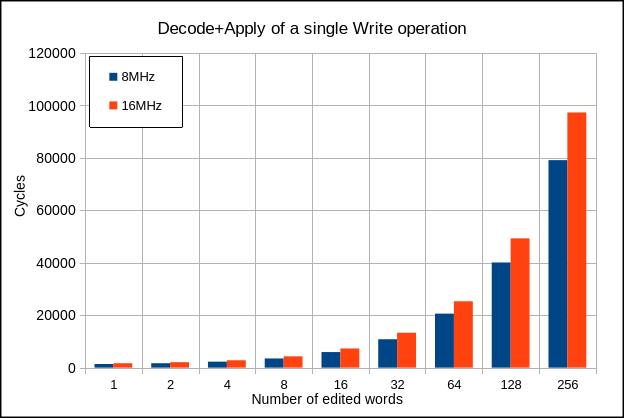
\includegraphics[width=\figurewidth]{img/W8vs16.png}
        \caption{Comparison of cycles required to decode and apply \textbf{Write} operations running at 8MHz and 16MHz.}
        \label{fig:w8vs16}
    \end{shaded}
\end{figure}

In previous works related to this research, various real-time deadlines have been targeted, such as Wahler et al. with 5ms \cite{dynUpdateFramework}, and Yaacoub et al. who measured an idle time of 3ms. Thus, these numbers ase used as target deadlines for the following discussion. Note that these deadlines may differ dramatically depending on the application and target system. 

The results of the simulated updates show that the DSU process benefits greatly from a higher clock frequency. 
\begin{figure}[!ht]
    \begin{shaded}
        \centering
        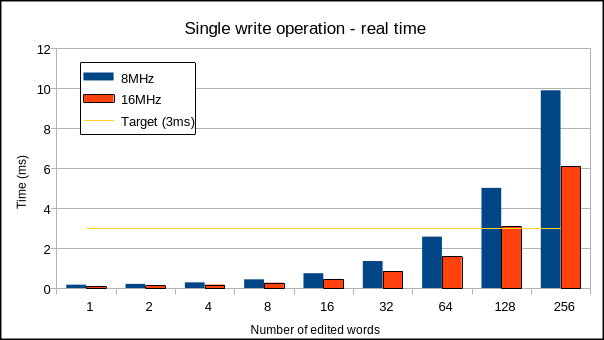
\includegraphics[width=\figurewidth]{img/W8vs16_rt.png}
        \caption{Comparison of real time required to decode and apply \textbf{Write} operations running at 8MHz and 16MHz.}
        \label{fig:s8vs16}
    \end{shaded}
\end{figure}

In figure \ref{fig:s8vs16}, the real-time performance of the update process is shown. The real-time performance is calculated by multiplying the number of cycles required to perform the update with the clock cycle time. As can be seen, the real-time performance of the update process is significantly improved when running at 16MHz, with the update process being on average $38.6\%$ faster. This is a significant improvement, and shows that the DSU process is feasible in a real-time system, even with the added overhead of wait states. Furthermore, using a linear regression, an estimated maximum size of a write operation was calculated to 124 words at 16MHz while still meeting the 3ms deadline. At 8MHz, this number is instead 75 words. This includes the decode phase, which the majority of time is spent in. Thus, if future work improves upon the decode phase, perhaps with more sophisticated encoding, it would certainly be possible to increase this limit.

\section{Proof of Concept Updates}
Firstly, to demonstrate the feasibility of the DSU process, a simple update was constructed which changes a single word in the binary image and makes the LED of the MSP430FR5994 blink at a different frequency. As expected from such a small update, the time it takes to perform the update is very short. The majority of time spent in the decoding phase, taking 1859 cycles, whereas the Apply phase only took 260. 

As a more interesting proof-of-concept, a larger update was constructed which changes the behaviour of the LED blinking and introduces new functionality to the application. The application pre-update blinks both LEDs on the launchpad at a fixed, synchronized frequency. The post-update application adds functionality to a button on the microcontroller. When pressed, the button changes the blinking frequency of one of the LEDs and makes them unsynchronized, thus providing a more complex update scenario which also has the benefit of being visibly verifiable. 
\begin{framed}
\noindent\begin{minipage}{.45\textwidth}
\begin{lstlisting}[
    caption={The interrupt service routine before DSU.},
    label={lst:pre_dsu_isr}
]
if (P5IFG & BIT5)
{ // Button 1 pressed
    update(diff);
}

P5IFG &= 0; // Clear interrupt flag
\end{lstlisting}
\end{minipage}\hfill
\noindent\begin{minipage}{.45\textwidth}
\begin{lstlisting}[
    caption={The interrupt service routine after DSU.},
    label={lst:post_dsu_isr}
]
if (P5IFG & BIT5)
{ // Button 1 pressed
    update(diff);
} 
if (P5IFG & BIT6)
{ // Button 2 pressed
    green_period += 1000;
}

P5IFG &= 0; // Clear interrupt flags
\end{lstlisting}
\end{minipage}
\end{framed}\hfill

The update took a total of 6151 cycles to complete at 8MHz, with the majority of the time spent in the decode phase. The update process was completed in 0.77ms, which is well within the 3ms deadline. This real-time performance is also expected to improve further when running at 16MHz, as previously discussed While this proof-of-concept is still relatively simple, requiring only a single \textbf{Shift}- and \textbf{Write} operation each, it demonstrates the potential of the DSU process. 


\section{Conclusion}
\section{Future Work}

\printbibliography

\end{document}